\section*{二、实验操作与原始数据}

\subsection*{1. 实验操作}

\subsubsection*{1.1 自组惠斯登电桥}

\begin{enumerate}
  \item 按惠斯登电桥原理连接检流计、电阻箱、待测电阻、比率臂和直流电源，电源电压为 $3.04\ \mathrm V$。
  \item 先选择 $k=R_1/R_2=1$，调节六旋钮电阻箱 $R_s$ 使检流计指零，记录 $R_s$。
  \item 在 $k=1$ 条件下分别取 $R_1=R_2=30.0\ \Omega$、$300.0\ \Omega$ 和 $3000\ \Omega$，改变 $R_s$ 为 $\Delta R_s=0.1\ \Omega$，记录检流计偏转格数，比较比率臂绝对值对灵敏度的影响，并选出灵敏度最高的桥臂设置。
  \item 采用选定的桥臂设置，交换 $R_x$ 与 $R_s$ 的位置，再次调平并记录 $R_s'$，按 $R_x=\sqrt{R_sR_s'}$ 计算待测电阻。
  \item 另取 $k=2$、$3$、$10$，重复交换法测量，以观察桥臂比率选择对结果的影响。
\end{enumerate}

\subsubsection*{1.2 Cu50 非平衡电桥}

\begin{enumerate}
  \item 按教材要求连接 FQJ 型非平衡直流电桥、Cu50 传感器和温控加热装置，将三个初始桥臂设置为 $R_1=R_2=R_3=50.0\ \Omega$。
  \item 实验现场室温约为 $24\,{}^\circ\mathrm C$，且不具备冰水混合物条件，因此未进行 $0\,{}^\circ\mathrm C$ 实际预调平衡；将功能开关置于“非平衡--电压”挡，按三桥臂均为 $50.0\ \Omega$ 的教材理想模型进行数据处理。
  \item 待室温示数稳定后按下 B、G 按钮，记录首组温度 $t$ 与非平衡电压 $U$。
  \item 从约 $25\,{}^\circ\mathrm C$ 开始加热，约每升高 $5\,{}^\circ\mathrm C$，待温度稳定后按下 B、G 按钮，记录非平衡电压 $U$ 及对应温度 $t$。
\end{enumerate}

\subsection*{2. 实验原始数据}

\begin{figure}[H]
  \centering
  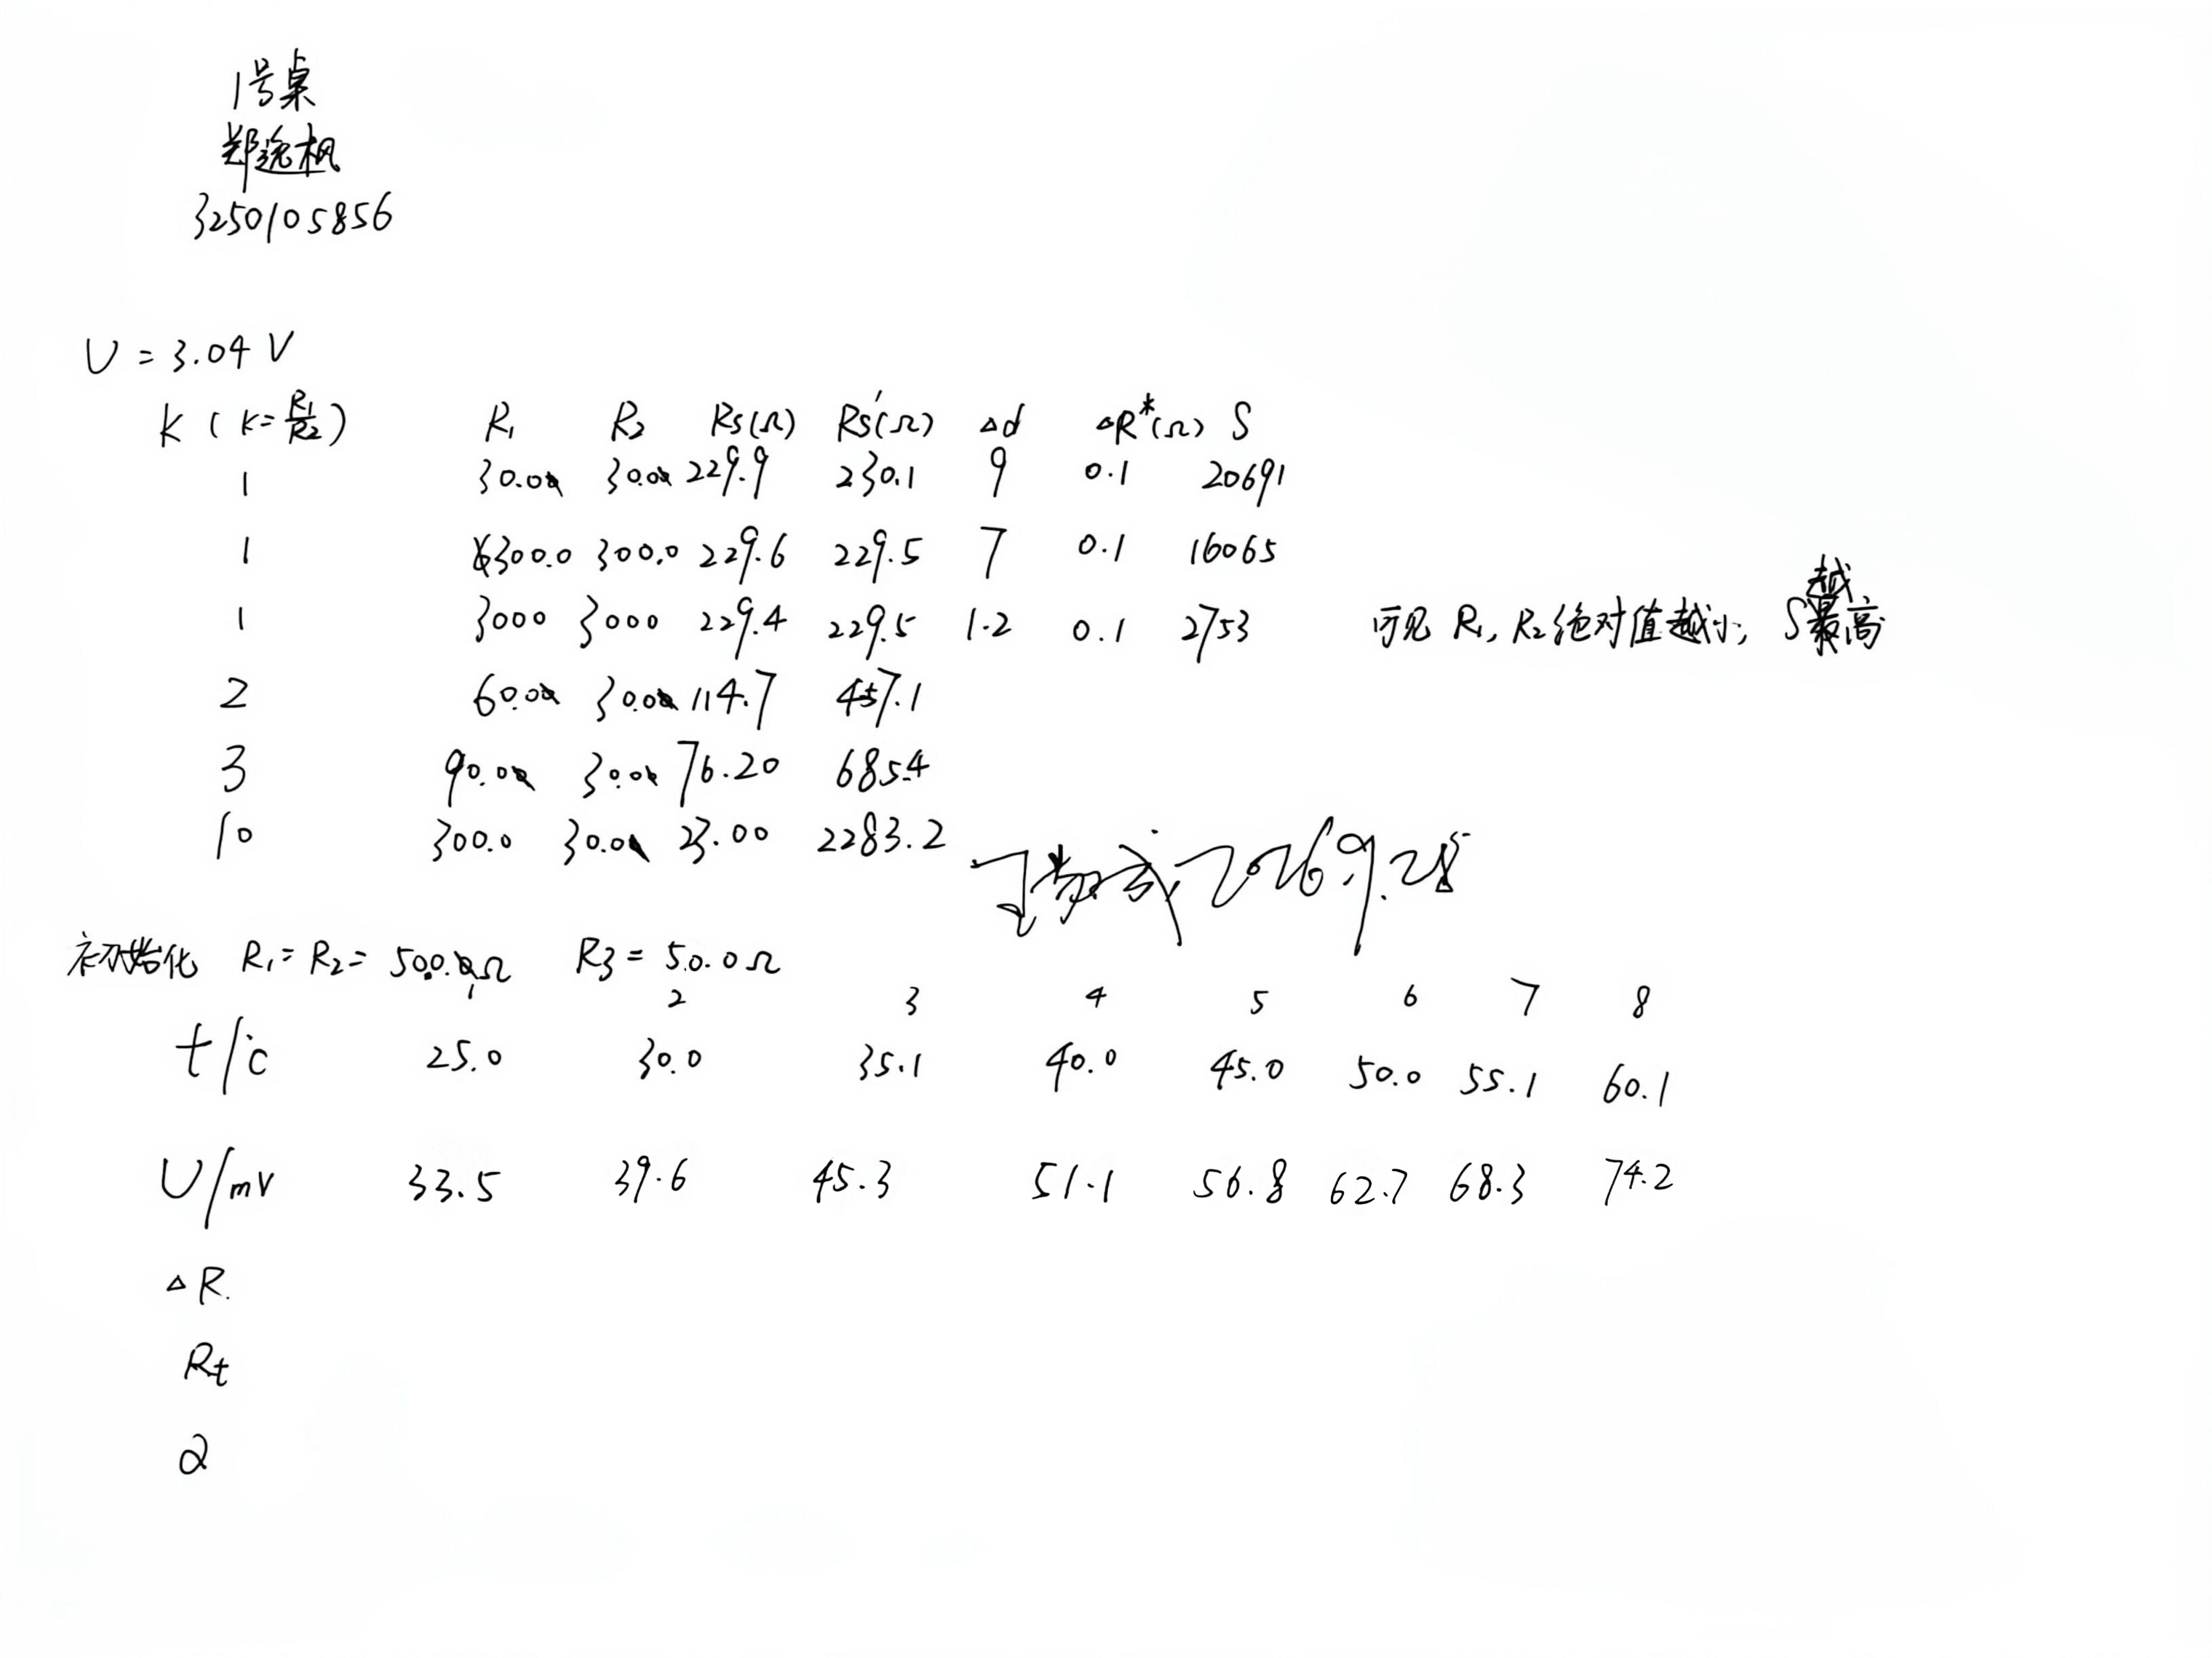
\includegraphics[width=\textwidth]{assets/raw-data.jpg}
  \caption{实验原始数据记录}
\end{figure}

\subsection*{3. 自组电桥原始数据}

\subsubsection*{3.1 比率臂绝对值与灵敏度}

以下三组均满足 $k=1$，其目的不是进行三次重复测量，而是在其他条件相同的情况下比较 $R_1$、$R_2$ 的绝对值对电桥灵敏度的影响。

\begin{table}[H]
  \centering
  \small
  \caption{比率臂绝对值与灵敏度原始数据}
  \begin{tabular}{ccccc}
    \toprule
    $R_1=R_2\,/\Omega$ & $R_s/\Omega$ & $R_s'/\Omega$ & $\Delta R_s/\Omega$ & $\Delta d$/格 \\
    \midrule
    30.0 & 229.9 & 230.1 & 0.1 & 9.0 \\
    300.0 & 229.6 & 229.5 & 0.1 & 7.0 \\
    3000 & 229.4 & 229.5 & 0.1 & 1.2 \\
    \bottomrule
  \end{tabular}
\end{table}

\subsubsection*{3.2 交换法与桥臂比率}

由上一节可知，$R_1=R_2=30.0\ \Omega$ 时电桥灵敏度最高，因此交换法结果中只保留该 $k=1$ 代表组，其余两组 $k=1$ 数据只用于灵敏度比较。

\begin{table}[H]
  \centering
  \small
  \caption{交换法与桥臂比率原始数据}
  \begin{tabular}{ccccc}
    \toprule
    $k$ & $R_1/\Omega$ & $R_2/\Omega$ & $R_s/\Omega$ & $R_s'/\Omega$ \\
    \midrule
    1  & 30.0  & 30.0 & 229.9 & 230.1 \\
    2  & 60.0  & 30.0 & 114.7 & 457.1 \\
    3  & 90.0  & 30.0 & 76.20 & 685.4 \\
    10 & 300.0 & 30.0 & 23.00 & 2283.2 \\
    \bottomrule
  \end{tabular}
\end{table}

\subsection*{4. Cu50 原始数据}

\begin{table}[H]
  \centering
  \small
  \caption{Cu50 温度与非平衡电压原始数据}
  \resizebox{\textwidth}{!}{%
  \begin{tabular}{c*{8}{c}}
    \toprule
    次数 & 1 & 2 & 3 & 4 & 5 & 6 & 7 & 8 \\
    \midrule
    $t/{}^\circ\mathrm C$ & 25.0 & 30.0 & 35.1 & 40.0 & 45.0 & 50.0 & 55.1 & 60.1 \\
    $U/\mathrm{mV}$ & 33.5 & 39.6 & 45.3 & 51.1 & 56.8 & 62.7 & 68.3 & 74.2 \\
    \bottomrule
  \end{tabular}}
\end{table}
